%!TEX root = ../main.tex
In this chapter, I introduce the SME model and the SME Implementation Language, SMEIL. I will also introduce CSP as well as \cspm{} and the FDR4 tool.

\section{Synchronous Message Exchange}
Since SMEIL is based on the SME model, I will give an introduction to SME to familiarize the reader with the SME model before introducing SMEIL.
\\

The development of SME was mainly driven by the need to provide a simple framework for programming a Field Programmable Gate
Array, FPGA. A lot of today's research focuses on General Purpose Graphical Processing Units, GPGPUs. The GPGPU has been extensively researched and different environments and tools have been implemented to give programmers the possibility of utilising all of its capabilities. However, FPGAs are a far better choice when it comes to energy sensitive applications, since FPGAs can achieve the same performance as a GPGPU but with lower energy consumption for some problems.

The FPGA has not been the subject of as much research as the GPGPU, and therefore when using FPGAs, the developer needs to design an integrated circuit on the gate level, which can be difficult and no longer common knowledge amongst programmers.
Unfortunately designing hardware is often a tedious task but with SME it becomes more accessible to design and implement hardware models.\\

The main target of SME is to give software developers a tool which provides the opportunity for the developer to program hardware but with a distance from the hardware details, so in a way, the development resembles the structures and semantics that is known from software development.
Thus the framework is based on a top-down approach rather than a bottom-up approach that is common in current hardware frameworks.
% Global synchronicity is fundamental when modeling hardware, but CSP does not support this. Even though CSP does enforce strict synchrony between communicating processes, there is no such semantic beging enforced on a global level. % TODO: Do I want to include this?

SME was first introduced in 2014 and after several iterations~\cite{Vinter2014, Vinter2015, Skovhede} now presents as a programming model, a simulation library, and VHDL code generators. The original idea was conceived following an attempt to create a hardware implementation of a vector processor, modeled in PyCSP~\cite{bjorndalen2007pycsp, vinter2009pycsp},
a Communicating Sequential Processes (CSP)~\cite{Hoare1978} library for Python.\\

The work was initially presented in the paper \textit{BPU Simulator}~\cite{Rehr2013} by M. Rehr, K. Skovhede, and B. Vinter, which introduced a high abstraction level simulation. Therefore the subject was explored more in detail in the master's thesis project \textit{Generation of FPGA Hardware
Specifications from PyCSP Networks}~\cite{Skaarup14} by E. Skaarup and A. Frisch. The results of this master's thesis made it clear that PyCSP could be used to model hardware, however the need to enforce global synchrony to the circuit resulted in a state explosion. The number of channels, for controlling the progress and for simulating the clock, became immense. Even simple circuits became overwhelmingly large.\\

The design approach within that project was to implement a clock process that would drive the circuit. This meant that each process would have to read the clock signal in, to ensure all processes listened to the clock. In order to avoid race conditions, the system had to be implemented with a two-way clock, the so-called \textit{tick}, \textit{tock} signals. Since deadlocks can happen in CSP, it was essential to implement deadlock prevention, which was done by adding channels with a single buffer element. This way, no process would end up in a deadlock. Figure \ref{fig:sme:clock_latch} shows how a simple CSP network would increase in complexity when modelled in the synchronous PyCSP model. It is clear how trying to use PyCSP for modelling synchronous hardware would result in extremely large and complex networks, which is not an ideal way to write hardware models.
\begin{figure}[h!]
\centering
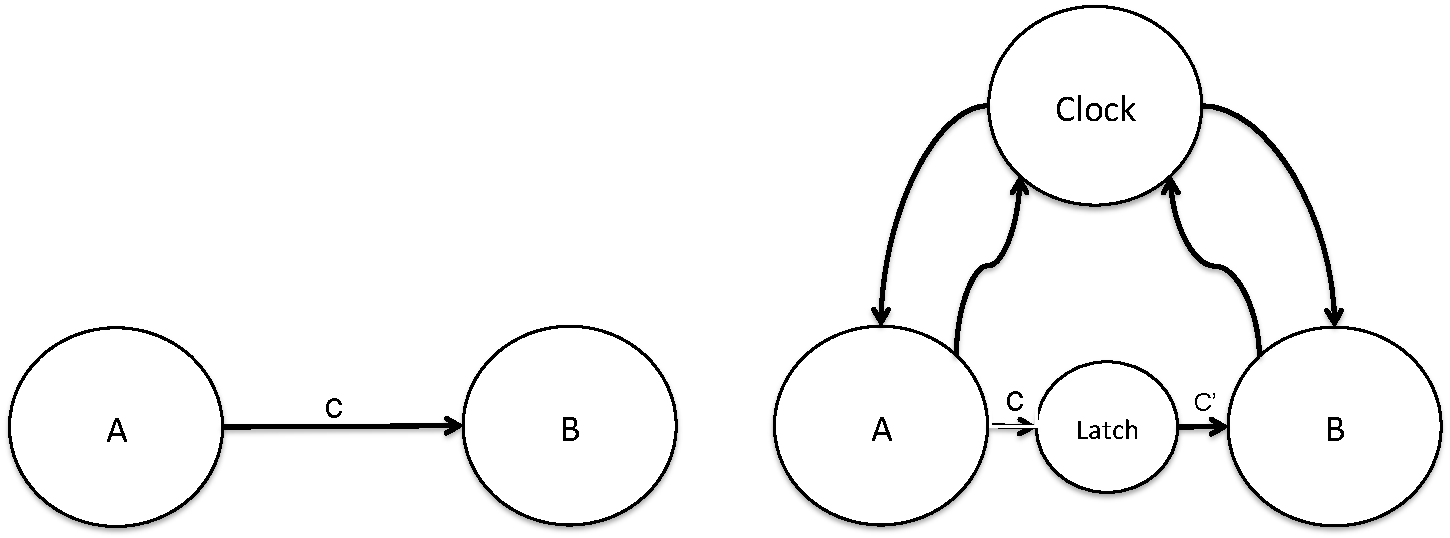
\includegraphics[width=10.0cm]{figures/clocked.pdf}
\caption{Enforcing global synchrony on a simple reader-writer network in CSP, resulting in a substantial increase in complexity. Figure from \cite{Vinter2014}.}
\label{fig:sme:clock_latch}
\end{figure}
\\\\
The advantage of using Python for processor simulation is the flexibility and simplicity of the language. It is easy to experiment with various ideas and structures, but with the increased complexity of the added clock process and clock-signal propagation, the advantages of Python seemed to diminish. Therefore the conclusion of the master's thesis project was that using PyCSP alone for building synchronous processor simulators was not ideal since the global clock was forced onto the CSP model. It was also concluded that external choice, which is a powerful and essential part of CSP, was not utilized in the globally synchronous approach. The thesis did, however, conclude that several other CSP concepts were fitting well with the hardware concepts, such as shared-nothing in CSP matching the structure of hardware communication.

After this attempt, it became clear that the structure of CSP was poorly suited for modeling clocked systems, and therefore it was decided to create the Synchronous Message Exchange framework, based on the CSP algebra. The idea was to only use the subset of the CSP algebra that provided beneficial functionality to hardware modeling which, most importantly, meant that external choice was omitted. However, the shared-nothing property of CSP showed to be very useful, since the network state could only be changed by process communication.
\\

% In SME the introduction of an implicit clock that eliminates the complexity caused by the model, described above, was imperative and is one of the key concepts hereof. The implicit clock removed the problems found by forcing the globally synchronous clock onto the CSP model. \\
In SME, a network is a combination of processes that are connected through buses. The processes communicate through a collection of signals in a bus, instead of CSP's synchronous rendezvous model, but retains the shared-nothing trait of CSP.
SME uses the term \texttt{bus} instead of \texttt{channel} to enforce the semantic correlation between the SME bus and a physical hardware signal bus.
The process communication is handled by a hidden clock which eliminates the complexity that arose from adding synchronicity to a CSP network. The combination of the hidden clock and the synchronous message passing between processes means that the SME model provides hardware-like signal propagation.

An SME clock cycle consists of three phases: it reads, executes, and writes as can be seen in Figure~\ref{fig:sme_process_flow}. The process is activated on the rising clock edge where it reads from the bus and then it executes and writes to the bus all in one clock cycle. Just before the rising edge of the clock, all signals are propagated on all buses which means that all communication happens simultaneously. Because of this structure, if a value is written by a process in cycle $i$, it is read by the receiving process in cycle $i+1$.

SME is able to detect read/write conflicts where multiple writes are performed to a single bus within the same clock cycle as well as reads from a signal that has not been written to in the previous clock cycle.

All data that are written to a bus, can be logged for each clock cycle and saved as Comma-Separated Values, CSV, which means that they can be used for validating the VHDL implementation with a VHDL tool. This eliminates the need to write separate VHDL tests which will improve developer productivity immensely.

% SME supports clock-multipliers which means that a clocked network can have components inside the network being clocked at a different rate than its own clock. The rate can be an integer multiplier from its own clock. This means that all components are clocked relative to its parent network and therefore the clock will not need any extra coordination. It does however, also mean that the inner components can only run faster than their parents.
% TODO: Do I really want this included?

% Since an SME network is a network that can be represented as a graph, a diagram tool have also been implemented for SME. It utilizes the Graphviz tool to generate a visual graph of the network. This means that the SME networks can be generated and drawn as a graph which can help with debugging.
%TODO: Also, it this something I really want to include?


\begin{figure}[!ht]
  \centering
  \begin{tikzpicture}[auto]
    \node[mycircle, text width=2cm, shape=rectangle] (read) {Read};
    \node[mycircle, text width=2cm, shape=rectangle] (execute) [below=0.5cm of read] {Execute};
    \node[mycircle, text width=2cm, shape=rectangle] (write)  [below=0.5cm of execute] {Write};

    \draw [myarrow] (read) -- (execute);
    \draw [myarrow] (execute) -- (write);
    \draw [myarrow] (write) |-([shift={(5mm,-5mm)}]write.south east)-- ([shift={(5mm,5mm)}]read.north east)-| (read);
  \end{tikzpicture}
  \caption{SME process flow for one clock cycle.}
  \label{fig:sme_process_flow}
\end{figure}
Since SME is based on CSP, all SME models have a
corresponding CSP model, and because of this property, we are able to create a transpiler translating SME models to \cspm{}.
The SME model is currently implemented as libraries for the general-purpose languages C\#~\cite{Skovhede}, C++~\cite{asheim2015}, and Python~\cite{asheim2016vhdl} and the language SMEIL which we will introduce further below. The Python and C\# libraries both have code generators for VHDL as well.
\subsection{SMEIL}
\label{sec:background_smeil}
With the different SME implementations, a need arose for a common intermediate language. SME Implementation Language (SMEIL) was developed as a Domain Specific Language (DSL) for SME, usable both as an Intermediate Language, IL, and as an independent implementation language. It is accompanied by the implementation, \texttt{LIBSME}. %TODO: Find the reference in truls paper.
SMEIL has a C-like syntax with a specialized type system that makes hardware modeling simple. In spite of its simplicity, SMEIL still provides hardware-specific functionality that is more difficult to create with general-purpose languages.

Programs written in SMEIL are run by using the libsme library, either by using the command line utility or through the provided API.
The different methods of using SMEIL are:\\
\begin{itemize}
    \item \textbf{Pure SMEIL simulation:} A pure SMEIL program is a network which does not depend on outside influence. This means that the network generates data itself and the only communication are between the processes defined in the network.
    \item \textbf{Co-simulation of SMEIL:} The original intent with SMEIL was to create an intermediate language which could be used together with the general-purpose language implementations of SME, which is called co-simulation. With co-simulation, a test bench can be generated as well as VHDL code.
    \item \textbf{Direct code generation:} A SMEIL program which does not need to simulate before generating VHDL. In this case, all types are constrained and all information needed for the code generation is in place. Because the simulation step is not executed, a VHDL test bench is also not automatically generated, since this happens in the simulation step.
\end{itemize}
An SMEIL module consists of the actual SMEIL program as well as import statements. SMEIL programs can be separated into modules which can then be imported into other SMEIL programs, creating a library-like structure and reusable components.\\

The two fundamental components of an SMEIL program are \texttt{process} and \texttt{network}. The process consists of variable and bus definitions, as well as the statements that are evaluated once for each clock cycle. The purpose of the \texttt{network} declaration is to define the relations between each entity in the program. A small example of the process and network syntax can be seen in Listing~\ref{lst:smeil_small_syntax_example} and a further introduction to the language can be found in Chapter \ref{chap:analysis}.\\

The SME model supports both synchronous and asynchronous processes. A synchronous process is run during every clock cycle and an asynchronous process are only run when receiving a signal on the input bus. Unfortunately, SMEIL does not currently support asynchronous processes.
\begin{listing}
\begin{minted}[escapeinside=&&, mathescape=true]{smeil_lexer.py:SMEILLexer -x}
proc addone (in inbus)
    bus outbus {
        val: int;
    };
{
    outbus.val = inbus.val + 1;
}

    &$\vdots$&

network net() {
    instance a of addone(b.outbus);
    instance b of ..
    &$\vdots$&
}
\end{minted}
\caption{Small example of process and network syntax in SMEIL.}
\label{lst:smeil_small_syntax_example}
\end{listing}
\subsubsection{SMEIL type system}
The SMEIL language is strongly, statically typed and has a simple type system that is checked at compile-time. The purpose of SMEIL is to be able to model hardware, and since hardware is static, it was important to create a type system that was capable of enforcing as many static invariants as possible.
Because of this, the only type coercion possible in SMEIL is between signed and unsigned integers. It is also the reason why only booleans can be used in conditionals.

The SMEIL type system differs from standard general-purpose languages mainly in the support for bit-precise types. General-purpose languages are typically targeted a CPU which consists of fixed-width registers which usually means that it can not work with data smaller than a byte. It is, however, an important part of modeling hardware to be able to define the exact widths of the buses, in order to optimise the hardware implementation. SMEIL supports unlimited-size integers as well as integers constrained to a specific bit-length. SMEIL also supports booleans, double and single precision floating point numbers as well as strings. Currently, floating-point numbers are supported in the SMEIL simulator but have not been extensively tested. The VHDL code generator does not support floating point numbers. \\
% Fixed length arrays of the types, mentioned above, are also supported.\\

In SMEIL buses are represented as channel names and their types, and since processes or networks can accept buses passed as parameters, it is important to ensure that no process or network is instantiated with a bus that does not contain the expected channels.
In the same way, it is essential to ensure that the directionality of the bus is enforced. When buses are passed as parameters, they are explicitly declared as either input or output bus. However, when defining a bus within a process it is not possible to define the directionality of the bus. Therefore the bus is defined as input or output based on their first use.
The type system of SMEIL is enforcing a set of rules that define how two buses are unified and the directionality of the bus, which ensures that unification and directionality problems, does not happen.
All types of declarations in SMEIL are private, except bus declarations. As mentioned above, they are used for establishing communication between processes and therefore needs to be a part of the public interface of a process or network.

\subsubsection{Simulating SMEIL programs}
For FDR4 to verify the networks within a reasonable timeframe, we have to constrain the state space that FDR4 has to search. Therefore, when translating SMEIL to hardware models, it is necessary to have all types in the program, constrained to a specific width. However, as mentioned before, SMEIL does support unlimited size integers. Since it can be difficult to define an optimal width when writing the SME model, it was necessary to provide both the support of the unlimited size integers while still being able to translate to hardware descriptions.

Therefore libsme provides a way to re-type the SME network based on the values observed during the simulation of the program.
During the simulation, the observed minimum and maximum value for all variables and channel are captured and saved along with the original value. SMEIL has been extended to include lower bounds for the purpose of this thesis.

After the simulation, these minimum and maximum values are then converted into SMEIL types large enough to hold the range.
The new SMEIL program, with the updated types and observed ranges, are then passed through the type checker in order to ensure that all constraints from the original program are still respected.

An example of this can be seen in Listing \ref{lst:smeil_restricted_types_and_ranges} where a unlimited size integer is re-typed to an integer of fixed size after the simulation.\\
\begin{minipage}[t]{.98\linewidth}
    % \centering
  \begin{minipage}[t]{0.45\linewidth}
    \begin{minted}{smeil_lexer.py:SMEILLexer -x}
proc A ()
    bus b {
        chan: int;
    };
    var c: i10;
{
    c = b.chan;
}
    \end{minted}
    \captionof{listing}{Example of unconstrained channel type before simulation.}
    \label{lst:unconstrained_smeil_type}
  \end{minipage}
  \hspace{0.5cm}
  \begin{minipage}[t]{0.45\linewidth}
    \begin{minted}{smeil_lexer.py:SMEILLexer -x}
proc A ()
    bus b {
        chan: i6 range 0 to 29;
    };
    var c: i10;
{
    c = b.chan;
}
    \end{minted}
    \captionof{listing}{Example of constrained channel type and range after simulation.}
    \label{lst:constrained_smeil_type}
  \end{minipage}
    \vspace{0.5cm}
   \captionof{listing}{Example of channel types before and after simulation. Example from \cite{smeil}.}
   \label{lst:smeil_restricted_types_and_rangesg}
   \vspace{1cm}
\end{minipage}
\subsubsection{Co-simulation}
Often when modeling hardware in Hardware Description Languages (HDLs) like VHDL or Verilog, code for testing and verifying are often written in the same language as the design itself. Unfortunately, the HDLs often does not have the functionality for generating proper simulation input. Using general-purpose languages for testing hardware models are useful since the range of available libraries are much larger.
Therefore the SMEIL simulator provides a simple language-independent API which enables SME implementations written for general-purpose languages to communicate with SME networks written in SMEIL, so-called co-simulation.
The big advantage of the SMEIL approach to co-simulation is that SME is used on both sides of the co-simulation and therefore can act as a single entity.
The PySME~\cite{pysme} library has been extended to support co-simulation with SMEIL, thereby providing the possibility of writing networks in PySME which can interact with SME networks written in SMEIL. Currently, only PySME has been extended with this but is expected to be implemented in the other SME implementations as well.
When simulating the SMEIL network, the compiler can record a trace of all communication between processes in the network. This trace file can then be used as a source for the VHDL test bench, which can be used to verify the generated VHDL code.

In Figure~\ref{fig:smeil_transpiler} the SMEIL transpiler structure can be seen.

\begin{figure}[!ht]
  \centering
  \begin{tikzpicture}[auto]
    \node[mycircle, minimum size=1.75cm, align=center, text width=1.75cm, font=\footnotesize]    (smeil)                                       {SMEIL};
    \node[myrectangle, text width=1.5cm, minimum height=1.0cm, inner sep=5pt, inner ysep=5pt] (csme)  [above left=-0.25cm and 1.5cm of smeil] {C\#SME};
    \node[myrectangle, text width=1.5cm, minimum height=1.0cm, inner sep=5pt, inner ysep=5pt] (pysme) [below left=-0.25cm and 1.5cm of smeil] {PySME};
    \node[myrectangle, text width=1.5cm, minimum height=1.0cm, inner sep=5pt, inner ysep=5pt] (vhdl)  [right=1.0cm of smeil]                {VHDL};

    \draw[myarrow] (csme)  -- (smeil);
    \draw[myarrow] (pysme) -- (smeil);
    \draw[myarrow] (smeil) -- (vhdl);
  \end{tikzpicture}
  \caption{SMEIL transpiler structure.}
  \label{fig:smeil_transpiler}
\end{figure}
\section{CSP}
\label{sec:csp_background}
Communicating Sequential Processes (CSP)~\cite{Hoare1978} is a process algebra that provides a way to express interaction between processes of concurrent systems.
CSP had a lot of influence in the design of the programming language Occam as well as the Go programming language and several others. As described in Chapter \ref{chap:related_work}, it was first introduced in 1976 by C.A.R Hoare but, not until 1984, did it develop into a process algebra. CSP is still a large research subject, and due to the tools available today, it is becoming increasingly more accessible for the general users.

CSP provides the possibility of describing systems in terms of message passing communication between independently operating processes. The \textit{sequential} part of the CSP name is not exactly applicable anymore, since the current version of CSP allows not only sequential processes, but also processes consisting of parallel compositions of other processes.
By using message passing between processes the language avoids certain problems that arise with the use of e.g shared variables.
It is possible to describe complex parallel structures with a few simple elements of the CSP algebra.

In CSP, a process is mainly defined by the way it can communicate with its external environment. An essential part of this communication is the \textit{alphabet} of possible communication events. This is the set of events that the process, and related processes, can use for communication. Events in CSP can only occur when both the process and the environment allow, but then they are instantaneous.

% TODO: Hvae I introduced TAPS before now? Because otherwise I have to introduce it here.
Here I give a brief introduction to the essential parts of CSP and structures that are used in TAPS, in order to give the reader a basic understanding to build on with \cspm{} and FDR. To learn more in-depth about CSP the reader is encouraged to seek out the books \textit{The Theory and Practice of Concurrency}~\cite{Roscoe1997} or \textit{Understanding Concurrent Systems}~\cite{Roscoe2010} by A. W. Roscoe.
\begin{itemize}
    \item \textbf{Prefix:} Given an event $a$ in the alphabet $\Sigma$, and a process $P$, $a \then P$ is the process which will communicate $a$ and then behaves like the process $P$. The process will wait indefinitely to communicate $a$. This is known as prefixing.
    The simplest CSP process possible is the \textit{STOP} process. It never does anything and never communicates and it is also known as the deadlocking process. The process $left \then right \then STOP$ is the process which communicates a left and a right before stopping. Another essential process is the \textit{SKIP} process which is the process that terminates successfully.
    \item \textbf{Recursion:} The process described above ends with \textit{STOP} and never resumes, but if I wish to have a process that performs the communication indefinitely, then recursion is used.
    $P_1 = left \then right \then P_1$ is the process that performs left and right in an infinite loop.
    \item \textbf{Events:} As described above, the only possible communication between processes are events within the defined alphabet. If $A \in \Sigma$ then the process $?x : A \then P(x)$ is the process which accepts an element $x$ of the set $A$ and then behaves like the process $P(x)$.
    It can often be valuable to have a "channel" to communicate values between processes. Therefore if $c$ is the channel, then $c?x : A \then P(x)$ is the process which receives an element $x$ on the channel $c$. This can also be written simply as $c?x \then P(x)$ where $A$ is the type of $c$. The "outputs" can be written in two ways, $c.x$ and $c!x$, which are equivalent. An example of a simple process receiving an element $x$ on the channel $c$ and outputs it again on the channel $c$ are $P = c?x \then c!x \then P$.
    \item \textbf{Guarded Alternative:} The guarded alternative provides the environment a choice between different actions. A simple choice statement could be $a \then P \barchoice b \then Q$ which gives the environment the possibility of choosing either to communicate $a$ and then behave as $P$ or communicate $b$ and then behave as $Q$.
    \item \textbf{Deterministic Choice:} Also called external choice is the operator which offers the environment the choice between two different processes. $(a \then P) \extchoice (b \then Q)$ is the process where the environment chooses to either perform event $a$ and then behave as the process $P$ or perform event $b$ and then behave as the process $Q$. This is completely the same as the guarded alternative example given above, and usually it is equivalent, however, some advanced uses of external choice might be hard to express simply with guarded alternative.
    \item \textbf{Nondeterministic Choice:} Also called internal choice, defines the choice between two processes but is not affected by the environment to make the decision.
    The process $(a \then P) \intchoice (b \then Q)$ can perform event $a$ or $b$ and then behave like the corresponding process, but it does not have to accept either. It is only required to accept one if the environment offers both of them.
    \item \textbf{Conditional Choice:} Conditional choices are also possible in CSP. Conditionals can be represented in different ways, which will be explained further in the \cspm{} section below. Hoares syntax for conditionals are $P \cond{b} Q$ which is the same as $\If b \Then P \Else Q$.
    \item \textbf{Interleaving:} This operator represents concurrent activity between two independent processes. $P  \interleave  Q$ defines a process behaving like $P$ and $Q$ simultaneously.
    \item \textbf{Generalised Parallel:} This operator represents concurrent activity between two independent processes but where the processes are required to syncronise on the set of events, defined in the operator. $ P  \parallel[a]  Q$ defines the process where $P$ and $Q$ must syncronise on event $a$ before the event can occur. All events not defined within the synchronisation can happen at any given time.
    \item \textbf{Alphabetised Parallel:} Imagine two processes that run in parallel. Some of the communication is with each other, but others are not. In this case, it is not possible to use the generalised parallel operator, since the processes also have to be able to communicate outside of the synchronisation. $P \parallel[X][Y] Q$ is the alphabetised parallel operator where $P$ is allowed to communicate to the set $X$ and $Q$ is allowed to communicate with the set $Y$. The two processes will have to synchronise on all communications within $X \cap Y$.
    \item \textbf{Hide:} This operator represents a process which performs any event from the defined set, but the event is hidden and becoming an internal event, a \textit{tau}($\tau$).
\end{itemize}

\subsection{\cspm{}}
In 1998 Bryan Scattergood introduced a machine-readable version of CSP, called \cspm. This language is an adaption and extension of the process algebra that Brookes, Hoare, and Roscoe introduced~\cite{Brookes1984}. The process algebra notation is extended with a functional programming language to be able to express CSP in a functional way, resulting in a language that can be used with tools and therefore providing a broader usability of CSP.

\cspm{} use the existing theory of CSP and in spite of being combined with a functional programming language, \cspm{} retains the idioms of CSP.
The main purpose of creating \cspm{} was not so it could be executed, like most programming languages. The main reason for creating \cspm{} was to provide an approach to describe parallel systems in a structure which can be automatically manipulated, with tools like FDR4.
% This also means that a program written in \cspm{} cannot be executed and simulated like a network can be simulated in SMEIL. In FDR4, the assertions defined in the program will be verified by looking through the entire state space of the program.\\

\subsubsection{Essentials of \cspm}
The basics of a \cspm{} script is to define the processes, their functionality, and the communication. \cspm{} supports sequences, sets, booleans, tuples, user-defined types, local definitions, pattern matching, and lambda terms.
\cspm{} does not enforce restrictions on the use of upper/lower-case letters in identifiers, although some standard conventions can be followed if needed. Some conventions define processes either all in capital letters or with an initial capital letter. Channels and function naming are typically all in lowercase lettering.\\

\cspm{} also supports integer arithmetics like addition, subtraction, product, quotient, remainder/modulus, and unary minus. Integer arithmetics are supported within a signed or twos-complement 32-bit representation.
Floating point numbers are currently not supported in \cspm. \\

\cspm{} provides several different built-in functions, like \texttt{concat(s)} or \texttt{elem(x,s)}, which both takes sequences as parameters, or \texttt{card(a)} and \texttt{union(a, b)} which are set functions. All of these functions are common in functional programming languages. \cspm{} support boolean \texttt{and}, \texttt{or}, \texttt{not} operations, equality operations as well as ordering operations and conditional expressions. In \cspm, all types except functions and processes can be compared with the equality operators. Ordering is defined for all but booleans or user-defined types. \\

Local definitions can be defined by wrapping them inside a \texttt{let within} statement. For example \texttt{P(n) = let (x,y) = n within x + y }, where \texttt{x} and \texttt{y} are local definitions.\\ Channel and datatype definitions can only be defined at top-level and therefore not in a \texttt{let within} statement. \\
\cspm{} provides support for lambda terms which have the syntax $\backslash \  x_1,...,x_n @\ x$. An example could be \texttt{f = \textbackslash x, y @ x \% y}. \\
It is simple and ideal to use pattern matching in a lot of cases in \cspm, similar to most functional programming languages. Case statements can be defined via pattern matching as well as comprehensions, communications etc. There are several rules that belong to pattern matching within \cspm{}, that will not be introduced here. For more information see the \cspm{} Reference Manual~\cite{Scattergood2011}.\\

In \cspm{} a channel is defined with the keyword \texttt{channel} and an identifier as a tag. Channels can be simple structures like \texttt{channel clock} or more complex like \texttt{channel c : \{0..10\}} which represents a channel $c$, that can communicate integers in the range of 0 through 10. A channel becomes an event when all necessary values have been provided. With channel \texttt{c}, the value \texttt{c.5} is of type \texttt{Event}. All events are members of the built-in data type \texttt{Events}. It is possible to define channels to be infinite, but when using \cspm{} in FDR4, it is not common use since FDR4 would run out of space due to the state space becoming too large.

\subsubsection{\cspm{} Processes}
In \cspm{}, processes are defined much like described in section \ref{sec:csp_background}, above. \texttt{SKIP} and \texttt{STOP} are defined the same, but external choice has a new syntax adapted to the functional language. Communications are done with the \texttt{?} and \texttt{!} operator, for example, \texttt{Proc(c) = c?x -> c!x -> Proc(c)}, is the process which receives an element on the channel \texttt{c} and outputs it on the same channel again.

Sequential composition is defined with a semicolon, for example, \texttt{P;Q} is first behaving like \texttt{P} until it terminates and then it behaves like \texttt{Q}.

External choice is defined with \texttt{P [] Q} and internal choice with \texttt{P |\textasciitilde| Q}. A boolean guard, \texttt{b \& P}, is the same as \texttt{if b then P else STOP}.
Generalised parallel is defined by \texttt{P [| A |] Q}, similar to how it is defined in the section above. It is worth noting that \texttt{P [|\{\}|] Q} is the same as using the interleave operator. \\
It is also possible to define alphabetised parallel, \texttt{P [A || B] Q}, which means that the set of events, \texttt{A}, are the events that \texttt{P} is allowed to perform and the set of events, \texttt{B} are the events allowed by \texttt{Q}.
%
% In \cspm{} when we wish to assert that some property hold for some process within the \cspm{} scripts. A basic assertion could be \texttt{assert 4 < 9}, but could also be used to express refinement checks, which is how FDR4 use assertions, which we explain further in the section below.\\

\subsection{FDR4}
\label{sec:background_fdr}
\textit{Note that the information represented in this section is based on the information published, which unfortunately does not include a lot of details about the internal workings of FDR4. I have assumed that the internal workings of FDR4 are similar to FDR3, which has been described in ~\cite{fdr}.}\\

Today, there exists several tools for formal verification. One of the currently most favored tools is the Failures-Divergences Refinement tool (FDR4). This tool is a CSP refinement checker that can analyze programs written in the machine-readable version of CSP, \cspm{}. Using the denotational models of CSP, \textit{traces}, \textit{failures}, and \textit{failures-divergences}, FDR4 is able to check if an implemented process refines a specification process. FDR4 also has the functionality of checking more properties than these models, like deadlock freedom or livelock freedom.

FDR was first released in 1991 and has since then been used both in academia and in the industry. The current version of FDR is the FDR4, which is a completely different system than the first version.
The FDR4 tool incorporates features like a \cspm{} type checker, a debugger as well as a built-in version of ProBE, the CSP process animator mentioned in Chapter \ref{chap:related_work}. FDR4 provides a parallel refinement-checking engine that can scale up linearly with the number of cores. This means that it can handle processes with a very large number of states in a reasonable time, which, along with compression, provides the possibility of verifying even larger problems. FDR4 also provide a cluster version, also providing verification of larger problems.\\

An assertion in FDR4 contains a specification process as well as an implemented process which we want to verify. For instance, \texttt{assert P [T= Q} means that we wish to assert if \texttt{Q} refines \texttt{P} according to the trace model.
FDR4 converts the two processes to a Labelled Transition Systems, LTS. A transition system consists of states and transitions between states which gives the opportunity of exploring the state space of the process.

FDR4 specifies the LTS further by using Generalised LST, GLTSs. A GLTS can have individual states being labeled with different properties, depending on the semantic model used for the refinement. For instance, if the trace model was used, then the states would be labeled with the traces in a GLTS.
FDR4 transforms both the specification process and the implementation process into GLTSs, which can then be checked for refinement. In order to be able to perform the verification, the specification GLTS is normalised, which has been extensively introduced in \cite{Roscoe1997}, but in short, the GLTS is transformed into a deterministic GLTS without any internal transitions or $\tau$ transitions. This can be an extensive operation, but since specification processes often are quite simple, this has proven to be the best approach.
After this, FDR4 is ready to check if the implemented process, transformed to a GLTS, refines the normalised specification GLTS, which is further introduced in section \ref{sec:refinement}. Since it is only necessary to normalise the specification process, the automatic refinement check becomes much more feasible than if it was necessary to normalise both. \\

FDR4 supports other compression functionalities besides normalisation, which can reduce the state space without changing the overall semantics of the process. This helps improve the runtime of the refinement checks. The reduction in state space is a crucial element of FDR4, since the state space quickly becomes overwhelmingly large, making the refinement check infeasible. The compression algorithms provide the possibility of verifying otherwise absurdly large problems.
These compression algorithms will not be further introduced in this thesis, but more information on these can be found in \cite{Roscoe2010}.

FDR4 also supports refinement of Timed CSP~\cite{REED1988249}~\cite{Armstrong2011} which is used within time-critical systems. \\

\subsubsection{Refinement}
\label{sec:refinement}
Refinement checking consists of searching through each of the GLTS, checking that all reachable states within the verification GLTS are compatible with every state within the normalised specification GLTS. It performs a breadth-first search, which has the advantage that when an error is found, the counterexample provided is the smallest possible. In each state, properties are checked according to the semantic model used. The refinement algorithm stores a set of states in order to keep count of what has been checked, what is currently being checked and what is left to be checked. FDR4 uses B-Trees to store data during refinement, and since version 3 of FDR, FDR3, the refinement can also be performed in parallel.
We will now introduce the three basic semantic models of CSP.
\paragraph{Traces model and refinement}
A trace is the sequence of communications between the process and the environment. Each element in the trace is the record of a single communication with the process, and a trace can be used to verify the correctness of a process in CSP. In the CSP algebra, refinement is written with the symbol $\refinedby$, and usually with a specific semantic model defined as well. Trace-refinement is specified by: \\
$$P \trefinedby Q \text{ if and only if } traces(P) \supseteq traces(Q)$$
This means that \textit{Q trace-refines P}, or in other words, that every finite trace of \textit{Q} is a trace of \textit{P}. \\
Some example are:\\
$traces(\STOP) = \{\emptyseq\}$\\
$traces(a \then \STOP) = \{\emptyseq, \seq{a}\}$\\
$traces((a \then \STOP)\extchoice (b \then \STOP)) = \{\emptyseq, \seq{a}, \seq{b}\}$.
% TODO: Maybe add an example with SKIP?
\paragraph{Failures model and refinement}
Traces are great at telling what the processes do, but they do have their limitations. For example, $a \then P \intchoice \STOP$ and $a \then P$ have the exact same trace, even though one has the possibility of \textit{STOP} and the other does not. This is why we, in some cases, need to look at not only what the process can do, but also what it can refuse to do. A refusal is a set of all the events that a process can fail to accept, no matter how long it is offered. A failure is a pair $(s, X)$ where $s$ is a trace and $X$ is the set of events that the process can refuse after the trace $s$.

\textit{failure(P)} is the set of all failures within the process \textit{P}. The GLTS is traversed and all routes through the graph are collected, while ignoring $\tau$ actions. This results in a trace and if the node at the end of each trace is stable, which means that there are no $\tau$ actions going out of it, this will give a failure since the node must refuse all actions that do not lead out of it. However, if the node has a $\tau$ action leading out from it, also called an unstable node, then it does not give a failure since the internal events will eventually happen.

An example of four different graphs can be seen in Figure \ref{fig:failures_graph}. It is assumed that the alphabet is \textit{\{a, b, c\}} and as can be seen, all stable notes have a subset of the alphabet next to it. These are the set of possible refusals for that node.
\begin{itemize}
    \item $P_1$ is a deterministic process, since it contains no $\tau$ events. A subset of the failures for this process are ($\emptyseq$, $\emptyset$), ($\emptyseq$, $\{c\}$), ($\seq{a}$, $\{a,c\}$) and ($\seq{a,b}$, $\{a,b,c\}$).
    \item $P_2$, $P_3$ and $P_4$ are nondeterministic due to the internal events.
\end{itemize}
We know that $$P \frefinedby Q \text{ if and only if } traces(P) \supseteq traces(Q) \text{ and } failures(P) \supseteq failures(Q)$$
When looking at Figure \ref{fig:failures_graph} it is clear that both $P_2$ and $P_3$ trace refines $P_1$, and they also have equivalent traces. In this example, only $P_2$ failure-refines $P_3$.
\begin{figure}[h]
\centering
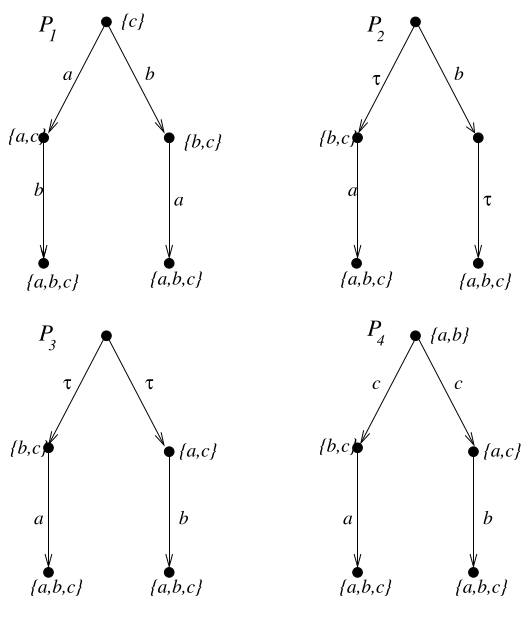
\includegraphics[width=0.6\textwidth]{figures/failures_graph.jpg}
\caption{Four different transition graphs and their refusal sets. Figure from ~\cite{Roscoe2010}.}
\label{fig:failures_graph}
\end{figure}
\paragraph{Failure-Divergences model and refinement}
Traces and failures are some very powerful models, however they do not account for divergence, which is addressed by the failure-divergence model. Divergence is a situation where a process performs an endless series of $\tau$ events. If a stable node in a transition graph, like the one in Figure \ref{fig:failures_graph}, went on to do endless internal actions, we would have a process that diverges. In the failure-divergences model, a process is represented by $(failures\bot(P), divergences(P))$. $divergences(P)$ represents the set of traces where $P$ can actually diverge afterwards. $failures\bot(P)$ represents the set of failures of $P$ extended by all the failures from the traces in $divergences(P)$, that is; $failures(P) \cup \{(s,X) | s \in divergences(P), X \subseteq \Sigma\}$.
In a transition graph, divergences occur where a process can reach itself with a number of $\tau$ events, i.e a $\tau$-loop.
% There are different ways to model divergence, and usually it is easier if divergence is assumed to be stict. Once a process has reached a point or trace where it might diverge, even though we do not actually know that it will go on forwver, there is no need to look at what else it could do. The assumption is that the process can do anything at all after that point, which is divergence strictness. It is possible to build models that does contain processes that diverge, but that are not divergence-strict. % TODO: I wrote this, but not sure if I think it is needed here.



% TODO: This does not belong here. Find out where it should go.
% For our current implementation of the transpiler, we can assert the ranges of the channel inputs, for example, we can automatically assert that the observed ranges, provided by the SMEIL simulation, and the possible input on the \cspm{} channels are not conflicting.
% In hardware, we would typically want to verify that the communication on a bus does not exceed a certain range or that the sum of multiple signals does not exceed a specific value. A bus might be able to carry other data than needed, and being able to model a circuit that can assert that the bus never carries other data than expected, is of great value.

% CSP was not initially developed for hardware modeling, and therefore it is not evident how to handle the clock cycle, which is an essential part of hardware modeling. When we transpile the SME network into \cspm{} the SMEIL simulation have provided the ranges of all values from the simulation and therefore all clock cycles. This means that when FDR4 asserts a property it asserts on all possible communication combinations for all the simulated clock cycles. Therefore, even though we are transpiling from an SME model, where the clock is crucial, we can simply translate ``one-to-one" from the SMEIL program and still get an accurate assertion on the properties.